\documentclass[10pt,a4paper]{article}
\usepackage[margin=20mm]{geometry}
\usepackage[T1]{fontenc}
\usepackage{amsmath,lmodern,graphicx,caption,booktabs}
\usepackage[hidelinks]{hyperref}
\setlength{\parindent}{0pt}
\setlength{\parskip}{5pt}
\captionsetup{font=small,labelfont=bf,hypcap=false}
\hypersetup{pdfauthor={Biswajit Jana},pdftitle={Ultraviolet knots and optical counterparts in NGC 4236}}
\begin{document}
{\LARGE\bfseries Ultraviolet knots and optical counterparts in NGC 4236\par}
\vspace{5pt}
{\large Biswajit Jana}\hfill November 2026

\textbf{Abstract.} We compare GALEX ultraviolet structure with Euclid DR1-Foundation VIS imaging near the inclined disk of NGC 4236. Of 182 UV peaks with usable VIS measurements and at least three local controls in strips away from the projected midplane, 143 exceed their local control median. Only two lie outside the adopted optical ellipse. An exploratory scan restricted to its exterior yields 23 peaks. Twenty exceed every local control and two have a VIS peak within $1''$ of the UV position. Gaia DR3 astrometry identifies one VIS peak with a foreground star. Narrow-band and broad-band imaging from SINGS has usable overlapping coverage at ten of the 23 UV positions. The evidence establishes projected UV--optical associations and leaves their relation to extraplanar ionised gas unresolved.

\section{Observations and methods}
Chy\.{z}y et al. (2007) mapped H$\alpha$ emission away from the disk. Young stars at those locations could ionise the gas locally. Ionising photons from stars elsewhere in the disk could also contribute. The first test here is whether Euclid resolves compact optical structure at the ultraviolet peaks. We use the background-subtracted MER VIS mosaic and flag image of Euclid tile 102161072 and FUV and NUV images from the GALEX Local Volume Legacy survey. These stacks and exposure and flag maps are archive products. We measure the UV peaks and the VIS excesses directly from them.

The initial search covers $\pm480''$ in major-axis position at PA $162^{\circ}$, with absolute minor-axis offsets of $60''$ to $180''$. At an adopted distance of 4.45~Mpc the latter are 1.29--3.88~kpc in projection. We use FUV coverage above 500~s. Candidates are local maxima in the difference of maps smoothed with Gaussians of standard deviation $1.8''$ and $12''$. Each peak exceeds five robust background scatter estimates in FUV and has a NUV excess above three within $3''$.

The VIS statistic is the strongest smoothed pixel within $2''$, measured relative to the median and robust scatter of a $3''$--$5''$ annulus. We require at least 90\% valid pixels inside $5''$ and at least three usable control positions drawn from shifts of $\pm15''$, $\pm30''$ and $\pm45''$ along the major axis. Controls avoid selected UV peaks by $8''$. In a separate exploratory scan, candidates and controls lie outside the adopted $21.9'\times7.2'$ optical ellipse, with $|x|\le480''$ and $|y|\le270''$ along the projected major and minor axes.

\section{Projected counterparts}
\begin{center}
\small
\begin{tabular}{lrrrr}
\toprule
Selection & UV peaks & With VIS and controls & Above median & Above all \\
\midrule
Projected strips & 190 & 182 & 143 & 80 \\
Exterior to optical ellipse & 23 & 23 & 23 & 20 \\
\bottomrule
\end{tabular}
\end{center}

Two strip peaks and 23 peaks from the restricted scan lie outside the nominal ellipse. Expanding both axes by 10\% moves both strip peaks inside, leaving 17 of the 23 exterior-scan peaks beyond the expanded boundary. Only two exterior candidates have a VIS maximum within $1''$ of the UV position. Nearby targets and controls can share optical structure, so the counts are descriptive.

\begin{center}
\begin{minipage}{.83\linewidth}
\centering
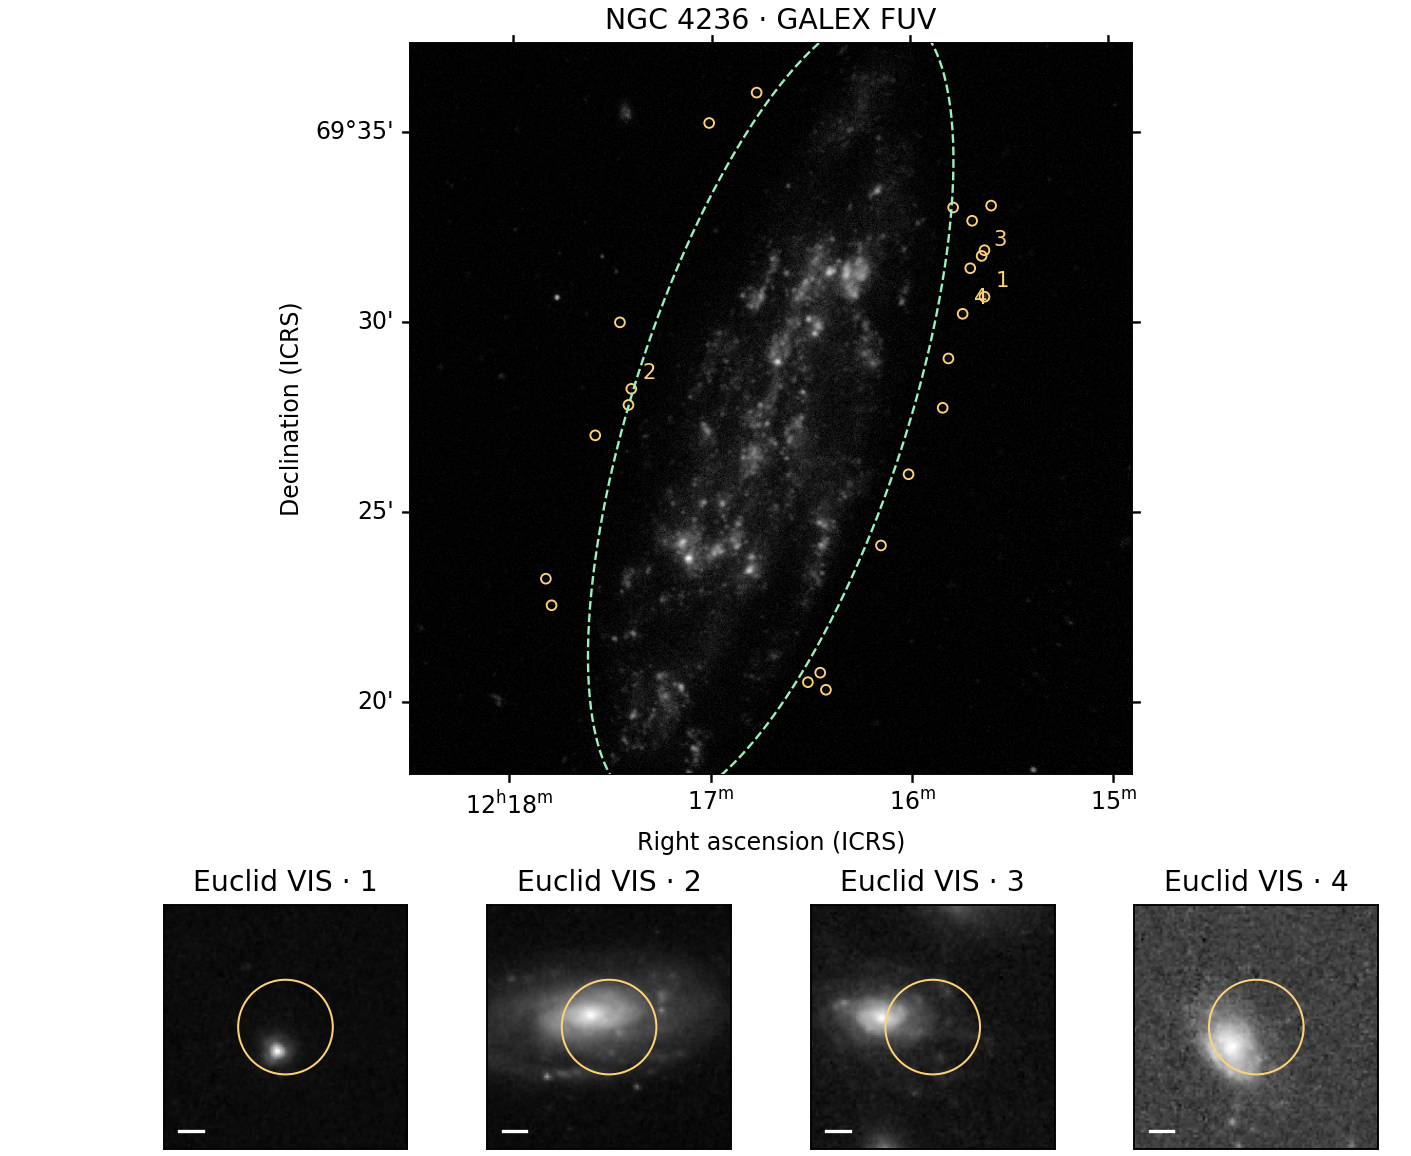
\includegraphics[width=\linewidth,height=51mm,keepaspectratio]{../analysis/outer_uv_vis.png}
\captionof{figure}{GALEX FUV field and Euclid VIS cutouts of the four brightest exterior peaks. Circles have a $2''$ radius. White bars span $1''$.}
\end{minipage}
\end{center}

\clearpage
\section{Foreground astrometry and narrow-band coverage}

\begin{center}
\begin{minipage}{.85\linewidth}
\centering
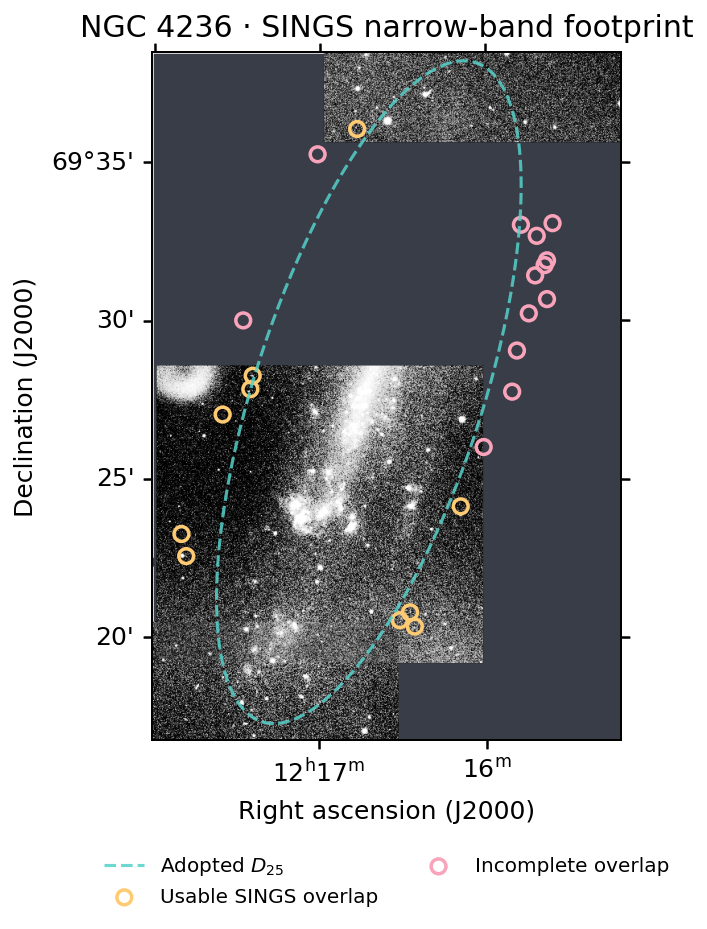
\includegraphics[width=\linewidth,height=63mm,keepaspectratio]{../analysis/sings_coverage.png}
\captionof{figure}{SINGS narrow-band footprint. Gold marks usable overlap in both SINGS bands and pink marks incomplete overlap. Grey marks narrow-band padding.}
\end{minipage}
\end{center}

We queried Gaia DR3 within $0.17^{\circ}$ of the centre, recovering 479 rows. Positions were propagated from J2016.0 to the GALEX observation on 24 January 2004 and to J2025.0 as a representative Euclid epoch. Three Gaia sources lie within $0.7''$ of a VIS peak and $3''$ of the respective GALEX peak. The same three matches survive VIS radii from $0.5''$ to $1.0''$. For a foreground flag we also require RUWE below 1.4 and either positive parallax or an absolute proper-motion component at least five times its formal uncertainty.

Candidate 23 passes this foreground test. Gaia DR3 1683447512960230528 lies $0.048''$ from the VIS peak and $1.93''$ from the UV peak. Its two proper-motion components are 9.7 and 54.9 times their formal uncertainties in absolute value. The two other Gaia matches are candidates 1 and 6. Candidate 1 has no significant motion or parallax and candidate 6 has no measured motion. The VIS association for candidate 23 demonstrates foreground contamination. The broader GALEX beam can include additional UV sources.

In the SINGS narrow-band and R-band pair, ten exterior positions have at least 90\% finite and nonzero pixels in a $6''$ radius in both images. Twelve have zero narrow-band coverage and one has partial overlap. The archived narrow-band image includes continuum and potentially [N\,II] emission. We measured its footprint only. These data provide no direct cross-identification with the H$\alpha$ clumps in the Chy\.{z}y et al. map, which used a different instrument.

\section{Interpretation}
A VIS peak near a GALEX position can trace a source unrelated to NGC 4236, as the Gaia match shows. A projected minor-axis offset in an inclined galaxy also leaves the source's physical height ambiguous. The remaining UV peaks lack demonstrated membership, and the current measurements do not constrain how abundant extraplanar young stars are.

{\small The \href{https://github.com/Biswajit1999/daily-astro-notebooks/tree/research/ngc4236-uv-optical/euclid-dr1-foundation/ngc4236-uv-optical}{study directory} contains the Gaia query, exact FITS IDs and checksums, coordinates, control statistics and code.\par}

{\footnotesize Chy\.{z}y et al. (2007), A\&A, 462, 933, \href{https://doi.org/10.1051/0004-6361:20065932}{doi}. Gil de Paz et al. (2007), ApJS, 173, 185, \href{https://doi.org/10.1086/516636}{doi}. Dale et al. (2009), ApJ, 703, 517, \href{https://doi.org/10.1088/0004-637X/703/1/517}{doi}. Lee et al. (2011), ApJS, 192, 6, \href{https://doi.org/10.1088/0067-0049/192/1/6}{doi}. ESA/Euclid \href{https://euclid.esac.esa.int/dr/dr1/expsup/}{DR1-Foundation documentation}. NASA/IPAC IRSA \href{https://doi.org/10.26131/IRSA414}{LVL} and \href{https://doi.org/10.26131/IRSA424}{SINGS}.\par}
\end{document}
